%%%%
% Преамбула: подключение необходимых пакетов
% Редактируйте осторожно!
%

\documentclass[hyperref={unicode}]{beamer}

\usepackage[utf8x]{inputenc}
\usepackage[english, russian]{babel}
\usepackage{color, colortbl}
\usepackage{rotating} 
\usepackage{graphicx}
\usepackage{algorithmic}

\usetheme[nosecheader]{PetrSU-CS}


%%%%
% Преамбула: основные параметры презентации
% Отредактируйте в соответствии с комментариями
%

\title[%
	% Краткое название работы не используется в этой презентации!
		Шаблоны страниц сайта для переводов
]{%
		% Полное название работы отображается на титульной странице
		Разработка шаблонов веб-страниц\\
		для веб-сервиса коллективных переводов
}

% Подзаголовком опишите тип работы:
% - Курсовая работа
% - Выпускная квалификационная работа бакалавра
% - Дипломная работа
% - Магистерская диссертация
\subtitle{Отчет о научно-исследовательской работе}

\author[%
		% Имя и фамилия автора работы отображаются на каждом слайде в нижнем колонтитуле
		Зименкова Софья
]{%
		% Имя, отчество и фамилия автора работы отображаются на титульном слайде
		Зименкова Софья Эдуардовна
}

\date[%
		% Дата защиты
		22.05.2023
]{%
		% Руководитель
		Научный руководитель: Д. Б. Чистяков
}

\institute[%
		% Краткое название организации не используется в этой презентации
		ПетрГУ
]{%
		% Полное название организации и подразделения
		Петрозаводский государственный университет\\
		Кафедра Информатики и Математического Обеспечения
}


%%%%
%
% Начало содержимого слайдов
%


%\begin{center}
%	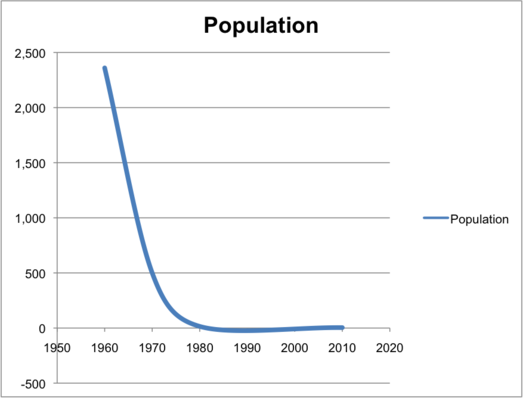
\includegraphics[width=0.4\textwidth]{images/pop.png}
%\end{center

\begin{document}

% Титульный слайд
\begin{frame}
\maketitle
\end{frame}


\begin{frame}
	
	\frametitle{Требования к сервису}
	Для организации эффективной работы коллектива переводчиков инструмент должен иметь следующие фукнции:
 \begin{itemize}
		\item загрузка текста и определение участников его перевода;
		\item разбиение исходного текста на главы и фрагменты;
		\item распределение задач и ролей между участниками перевода;
		\item сихнронизация материалов и прогресса между участниками перевода;
		\item выбор и утверждение наилучшего варианта перевода;
		\item выгрузка итогового текста.
	\end{itemize}
	
	Эти функции удобно реализовать с помощью веб-сервиса, поэтому инструмент будет реализован в виде сайта.
\end{frame}


\begin{frame}
	\frametitle{Цель и задачи}
	\begin{block}{Цель работы}
		%Разработать основу веб-сервиса для коллективных переводов.
		Разработка шаблонов веб-страниц для описанного сервиса.
	\end{block}
	\begin{block}{Задачи}
	\begin{itemize}
		\item исследовать существующие веб-сервисы и сделать выводы о необходимом функционале и подходящем дизайне интерфейса;
		\item изучить существующие инструменты и технологии для разработки веб-страниц, выбрать наиболее подходящие для реализации проекта;
		\item разработать удобные и визуально привлекательные шаблоны веб-страниц.
	\end{itemize}
	\end{block}
\end{frame}


\begin{frame}
	\frametitle{Необходимые данные для разработки веб-страниц}
	\begin{block}{Определение}
		\textbf{UX} (англ. user experience — «пользовательский опыт») — взаимодействие пользователя с интерфейсом, удобство интерфейса. \\
		\textbf{UI} (англ. user interface — «пользовательский интерфейс») — оформление сайта: сочетания цветов, шрифты, иконки и кнопки.
	\end{block}
	В отсутствии необходимого опыта или образования в сфере веб-дизайна, разработчик может использовать готовые библиотеки компонент или фреймворки.
	\begin{block}{Определение}
	\textbf{Фреймворк} (англ. framework — «структура») — готовый набор инструментов, помогающий разработчику быстро создать продукт.
	\end{block}
	Также разработчику стоит изучить другие приложения/сервисы, чтобы понять, какой интерфейс удобен для пользователя.
\end{frame}


\begin{frame}
	\frametitle{Примеры существующих веб-сервисов для коллективных переводов}
	\begin{itemize}
		\item Crowdin.com
		\begin{itemize}
			\item[+] Множество инструментов, форматов файлов;
			\item[--] Локализация ПО и документации, неинтуитивность, платный сервис.
		\end{itemize}
		\item Notabenoid.org
		\begin{itemize}
			\item[+] Разные форматы файлов, удобный дизайн, публичные проекты;
			\item[--] Устаревший сервис, мало инструментов, закрытый сервис.
		\end{itemize}
		\item Transifex.com
		\begin{itemize}
			\item[+] Множество инструментов, форматов файлов;
			\item[--] Узконаправлен, платный сервис.
		\end{itemize}
	\end{itemize}
\end{frame}


\begin{frame}
	\frametitle{Примеры существующих веб-сервисов для коллективных переводов}
	\begin{itemize}
		\item Translatewiki.net
		\begin{itemize}
			\item[+] Удобный, простой, открытый, бесплатный;
			\item[--] Только перевод вики-страниц.
		\end{itemize}
		\item Weblate
		\begin{itemize}
			\item[+] Поддерживает частые обновления оригинала, GitHub, удобные инструменты;
			\item[--] Узконаправлен, платный сервис, не подходит любителям.
		\end{itemize}
	\end{itemize}
	Вывод:
	\begin{itemize}
		\item Минималистичный дизайн интерфейса;
		\item Разделение исходного текста на фрагменты;
		\item Поддержка разных форматов входных данных;
		\item Система ролей и голосования;
		\item Универсальность и доступность.
	\end{itemize}
\end{frame}


\begin{frame}
	\frametitle{Инструменты и технологии}
	\begin{block}{Определение}
		\textbf{HTML} (HyperText Markup Language) — язык разметки, используемый для структурирования и отображения веб-страницы и ее контента.
	\end{block}
	\begin{block}{Определение}
		\textbf{CSS} (Cascading Style Sheets) — язык таблицы стилей, используемый для применения стилей к элементам в документах HTML.
	\end{block}
	Несколько вариантов выбора инструментов:
	\begin{itemize}
		\item \textbf{Bootstrap};
		\item Tailwind;
		\item Material-UI;
		\item Foundation;
		\item UIkit.
	\end{itemize}
\end{frame}


\begin{frame}
	\frametitle{Разработка шаблонов веб-страниц}
	\begin{block}{Инструменты}
		HTML5, Bootstrap v5.3
	\end{block}
	Листинги страниц доступны по ссылке:\\
	\texttt{https://github.com/ipaingo/DesmanTranslate}
	
	Пример использования Bootstrap:\\
	\begin{center}
	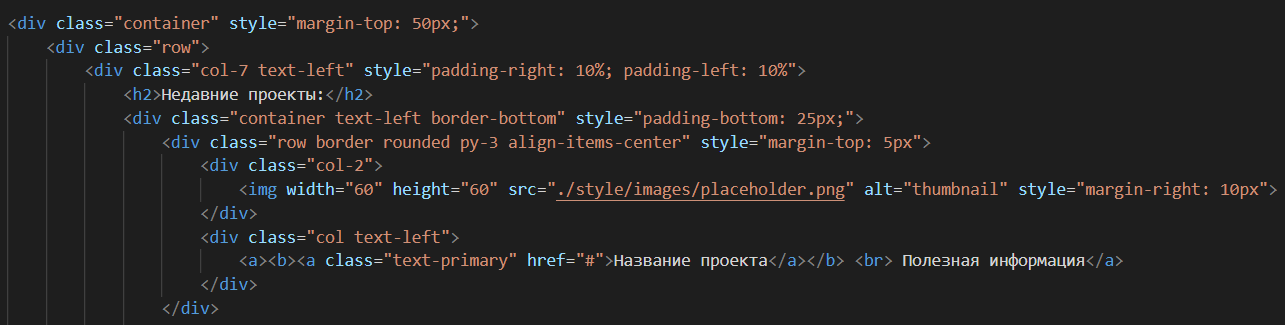
\includegraphics[width=\textwidth]{images/code.png}
	\end{center}

\end{frame}


\begin{frame}
	\frametitle{Пример внешнего вида страницы}
	\begin{center}
	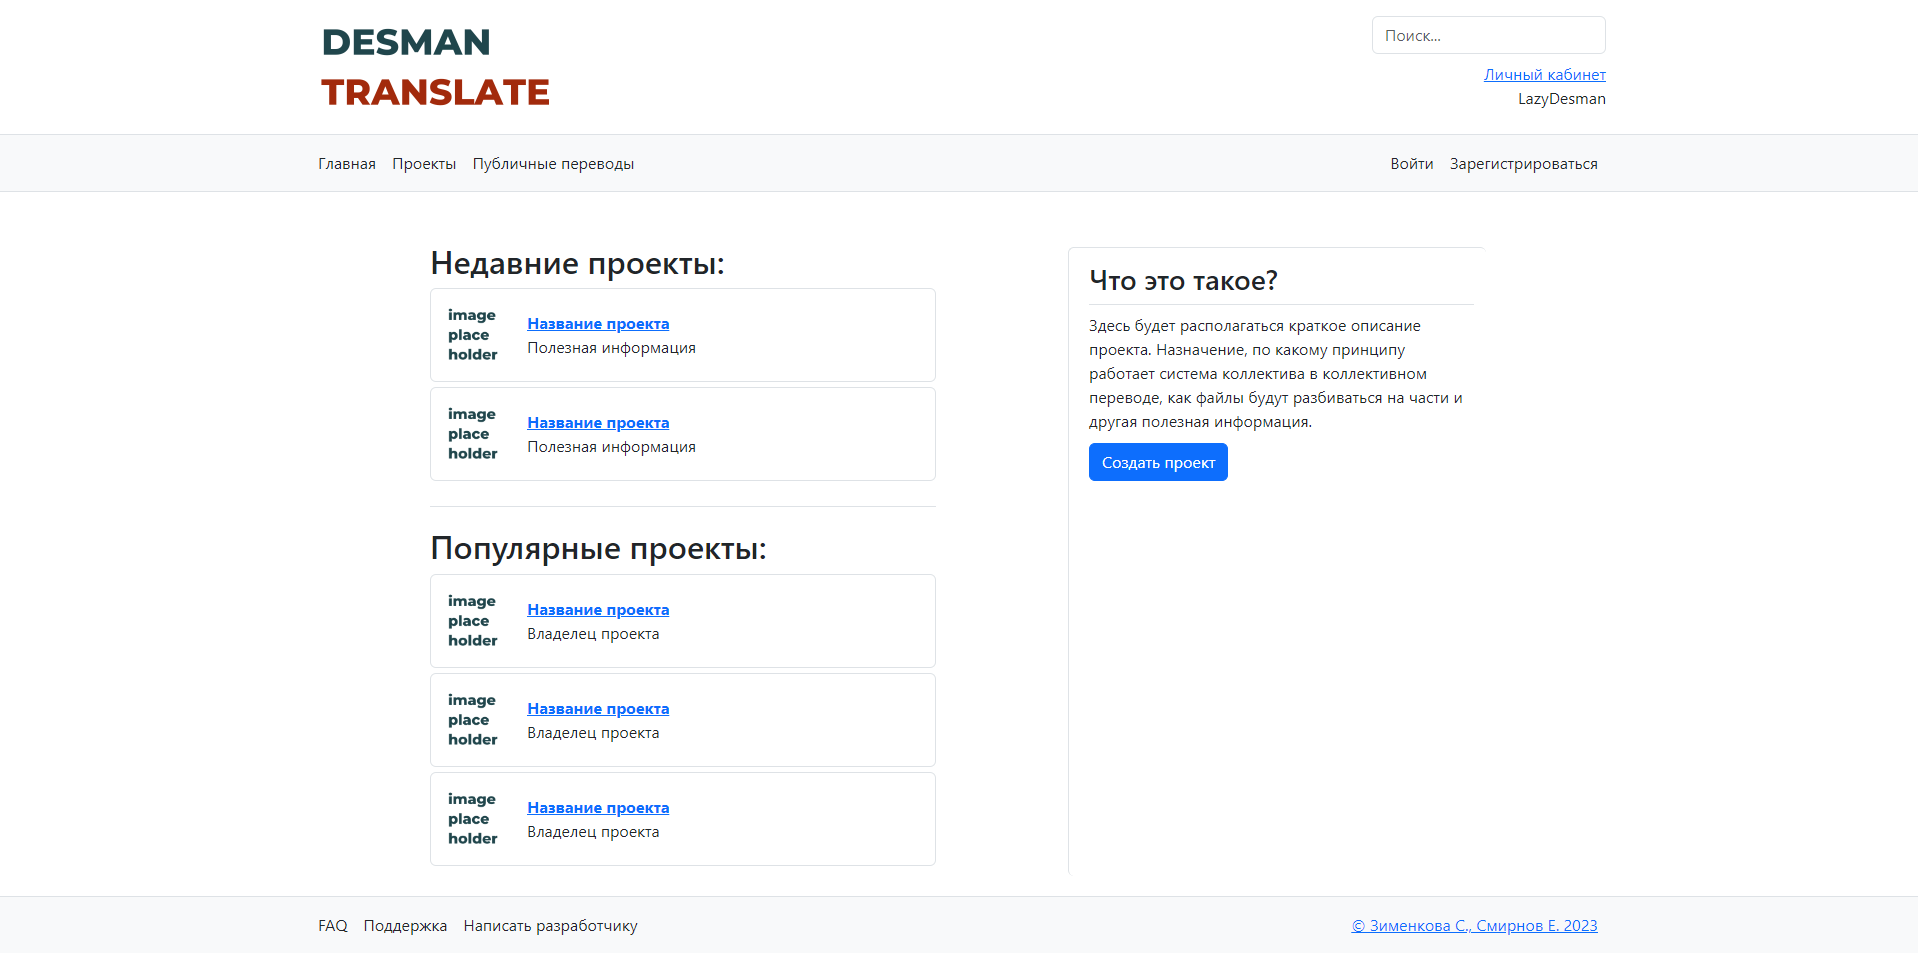
\includegraphics[width=\textwidth]{images/index.png}
	\end{center}
\end{frame}


\begin{frame}
	\frametitle{Пример внешнего вида страницы при изменении размера окна}
	\begin{center}
	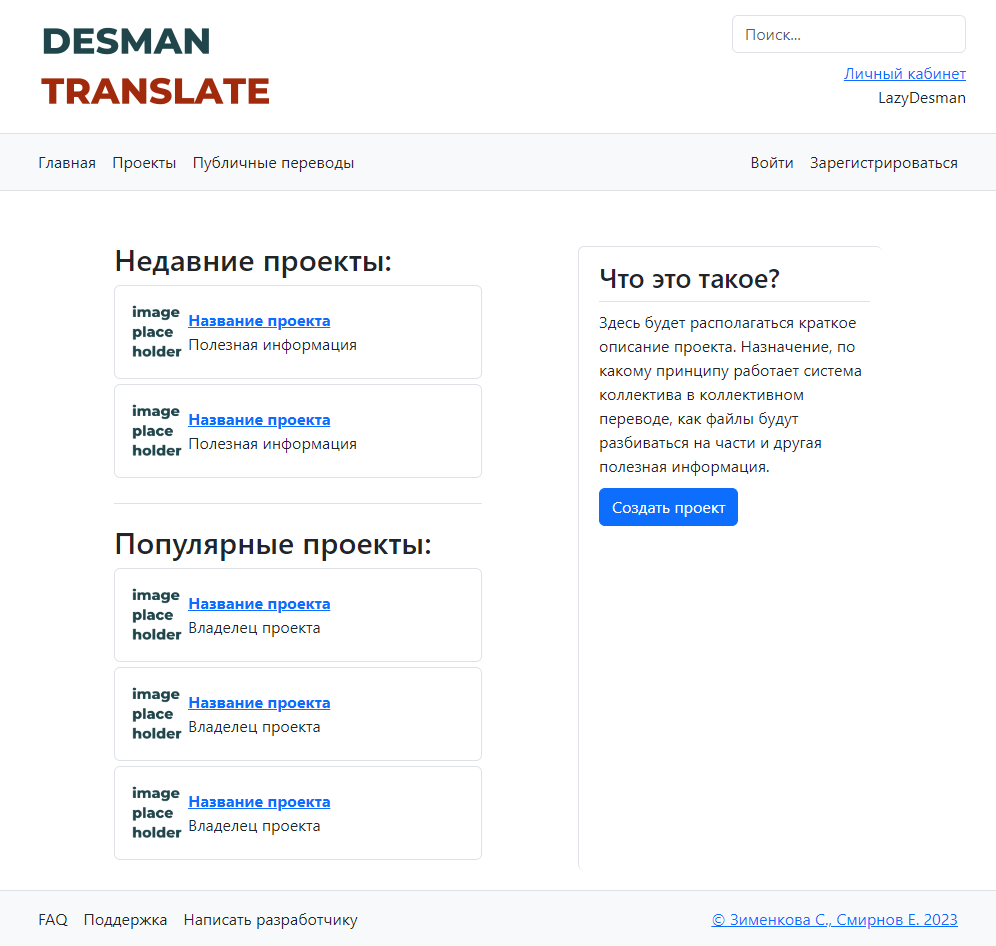
\includegraphics[width=0.6\textwidth]{images/smallindex.png}
	\end{center}
\end{frame}


\begin{frame}
	\frametitle{Пример внешнего вида страницы проекта}
	\begin{center}
	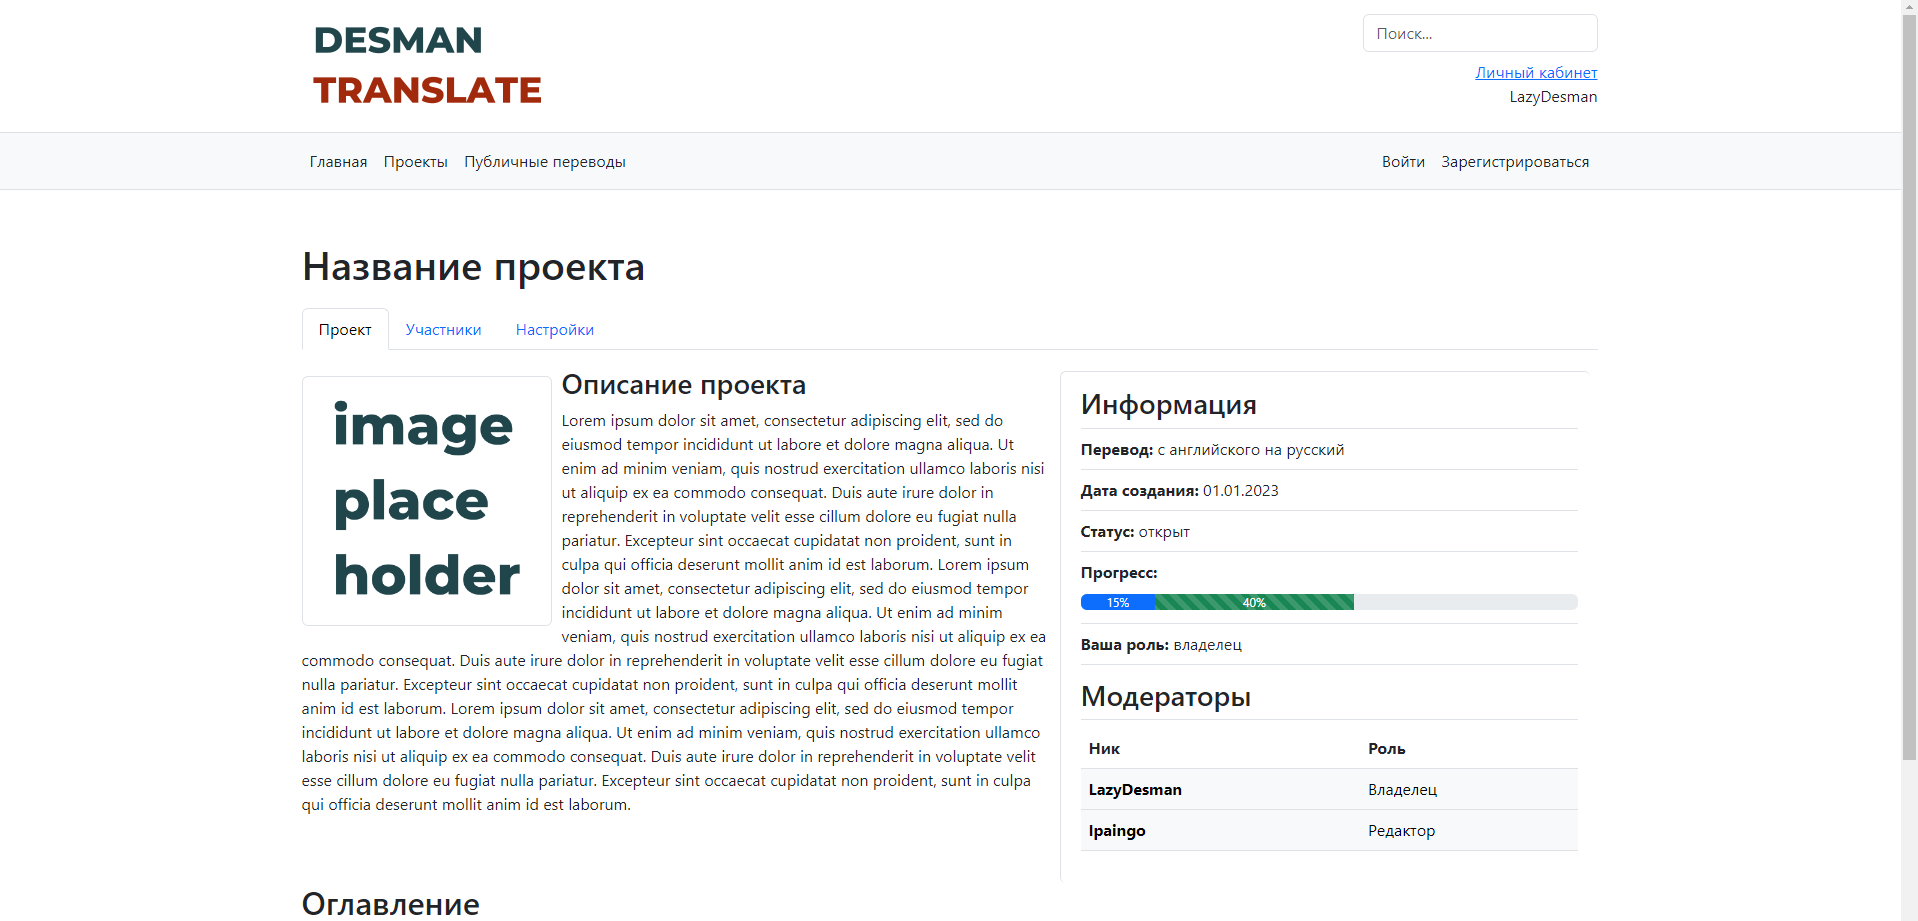
\includegraphics[width=\textwidth]{images/projectpage1.png}
	
\includegraphics[width=\textwidth]{images/projectpage2.png}
	\end{center}
\end{frame}

% % Пример слайда содержащего код
% \begin{frame}[fragile]
% 	
% 	\frametitle{Алгоритм расчета поголовья бобров}
% 	\framesubtitle{(оформляем фрагмент исходного кода или псевдокода)}
	
% 	\begin{verbatim}
% 		цикл для всех водоемов
% 			цикл для всех хаток
% 				если хатка не брошена, то
% 					sum += количество бобров в текущей хатке
% 				конец условия
% 			конец цикла по хаткам
% 		конец цикла по водоемам
% 	\end{verbatim}
	
% \end{frame}

 % Пример заключительного слайда
 \begin{frame}
 	\frametitle{Заключение}
	
 	Полученные результаты:
	
 	\begin{itemize}
 		\item Исследованы существующие сервисы для осуществления коллективных переводов, их преимущества и недостатки;
 		\item Изучены доступные инструменты и технологии для создания веб-страниц;
 		\item Выбраны оптимальные для реализации описанного проекта инструменты;
 		\item Реализованы HTML-файлы с шаблонами веб-страниц, которые упростят и ускорят дальнейшую разработку. 
 	\end{itemize}
	
\end{frame}

 \begin{frame}
 	\frametitle{}
\begin{center}
 {\Large\mbox{}Спасибо за внимание!}
\end{center}
 \end{frame}
\end{document}
